\documentclass{article}
\usepackage{fancyhdr} % Required for custom headers
\usepackage{lastpage} % Required to determine the last page for the footer
\usepackage{extramarks} % Required for headers and footers
\usepackage[usenames,dvipsnames]{color} % Required for custom colors
\usepackage{graphicx} % Required to insert images
\usepackage{listings} % Required for insertion of code
\usepackage{courier} % Required for the courier font
\usepackage{lipsum} % Used for inserting dummy 'Lorem ipsum' text into the template
\usepackage{caption}
\usepackage{subcaption}
\usepackage{amsmath}
\usepackage{amsfonts}
\usepackage{amssymb}
\usepackage{epstopdf}
\usepackage{placeins}
\usepackage{color} 
\usepackage{fancyvrb} 
\usepackage{setspace}
\usepackage{array}
\usepackage[numbered]{bookmark}
\usepackage{tikz}
\usepackage{pgfplots}
\usepackage[absolute,overlay]{textpos}
\usetikzlibrary{calc, angles,quotes}
\usetikzlibrary{pgfplots.fillbetween, backgrounds}
\usetikzlibrary{positioning}
\usetikzlibrary{arrows}
\usetikzlibrary{pgfplots.groupplots}
\usetikzlibrary{arrows.meta}
\usetikzlibrary{plotmarks}
\usetikzlibrary{decorations.markings}

\usepgfplotslibrary{groupplots}
\pgfplotsset{compat=newest} 
%\pgfplotsset{plot coordinates/math parser=false}
\DeclareGraphicsExtensions{.pdf,.png,.jpg}
\graphicspath{{figs/}}

\definecolor{matlabcomment}{RGB}{34,139,34}

\pgfmathdeclarefunction{gauss}{1}{%
	\pgfmathparse{1/(sqrt(2*pi))*exp(-((#1)^2)/2)}%
}

\pgfmathdeclarefunction{laplacian}{2}{%
	\pgfmathparse{1/(#2*2)*exp(-(abs(x-#1))/(#2))}%
}

\pgfmathdeclarefunction{pretty_func}{1}{%
	\pgfmathparse{cos(deg(#1/2)) - sin(deg(#1)) + cos(deg(#1/2)-45) - sin(deg(#1/4)-154)}%
}

\pgfplotsset{
	dirac/.style={
		mark=triangle*,
		mark options={scale=2},
		ycomb,
		scatter,
		visualization depends on={y/abs(y)-1 \as \sign},
		scatter/@pre marker code/.code={\scope[rotate=90*\sign,yshift=-2pt]}
	}
}

\def\thickness{very thick}

\tikzset{
amark/.style 2 args={
	decoration={             
		markings, 
		mark=at position {0.5} with { 
			\arrow{stealth},
			\node[#2] {#1};
		}
	}, \thickness,
	postaction={decorate}
},
earlymark/.style 2 args={
	decoration={             
		markings, 
		mark=at position {0.25} with { 
			\arrow{stealth},
			\node[#2] {#1};
		}
	}, \thickness,
	postaction={decorate}
},
latemark/.style 2 args={
	decoration={             
		markings, 
		mark=at position {0.8} with { 
			\arrow{stealth},
			\node[#2] {#1};
		}
	}, \thickness,
	postaction={decorate}
},
zpath/.style={
	decoration={             
		markings, 
		mark=at position {0.5} with { 
			\arrow{stealth},
			\node[#1] {$z^{-1}$};
		}
	}, \thickness,
	postaction={decorate}
},
terminal/.style 2 args={draw,circle,inner sep=2pt,label={#1:#2}},
}


\tikzset{
	invisible/.style={opacity=0},
	visible on/.style={alt={#1{}{invisible}}},
	alt/.code args={<#1>#2#3}{%
		\alt<#1>{\pgfkeysalso{#2}}{\pgfkeysalso{#3}} % \pgfkeysalso doesn't change the path
	},
}

\newcommand\PlotSampledSpectrum[4]{%
	\def\fs{#2}%
	\def\fmax{#3}%
	\def\ros{#4}%
	\input{#1}%
}

\pgfmathdeclarefunction{invgauss}{2}{%
	\pgfmathparse{sqrt(-2*ln(#1))*cos(deg(2*pi*#2))}%
}

\tikzset{
	declare function={
		sinc(\x) = (and(\x!=0, 1) * (sin(deg(pi*\x))/(pi*\x)) +
		(and(\x==0, 1) * 1);
	}
}

\DeclareMathOperator{\E}{\mathbb{E}} % expectation

\newcommand\SimpleSys[4]{%
	\def\xin{#2}%
	\def\Hz{#3}%
	\def\yout{#4}
	\input{#1}%
}

% Margins
\topmargin=-0.45in
\evensidemargin=0in
\oddsidemargin=0in
\textwidth=6.5in
\textheight=9.0in
\headsep=0.25in

\linespread{1.2} % Line spacing

% Set up the header and footer
\pagestyle{fancy}
\lhead{\hmwkAuthorName} % Top left header
\chead{\hmwkTitle} % Top center head
\rhead{\hmwkClass} % Top right header
\lfoot{} % Bottom left footer
\cfoot{} % Bottom center footer
\rfoot{Page\ \thepage\ of\ \protect\pageref{LastPage}} % Bottom right footer
\renewcommand\headrulewidth{0.4pt} % Size of the header rule
\renewcommand\footrulewidth{0.4pt} % Size of the footer rule

%\setlength\parindent{0pt} % Removes all indentation from paragraphs
\definecolor{MyDarkGreen}{rgb}{0.0,0.4,0.0} % This is the color used for comments
\lstloadlanguages{Perl} % Load Perl syntax for listings, for a list of other languages supported see: ftp://ftp.tex.ac.uk/tex-archive/macros/latex/contrib/listings/listings.pdf
\lstset{language=Perl, % Use Perl in this example
        frame=single, % Single frame around code
        basicstyle=\small\ttfamily, % Use small true type font
        keywordstyle=[1]\color{Blue}\bf, % Perl functions bold and blue
        keywordstyle=[2]\color{Purple}, % Perl function arguments purple
        keywordstyle=[3]\color{Blue}\underbar, % Custom functions underlined and blue
        identifierstyle=, % Nothing special about identifiers                                         
        commentstyle=\usefont{T1}{pcr}{m}{sl}\color{MyDarkGreen}\small, % Comments small dark green courier font
        stringstyle=\color{Purple}, % Strings are purple
        showstringspaces=false, % Don't put marks in string spaces
        tabsize=5, % 5 spaces per tab
        %
        % Put standard Perl functions not included in the default language here
        morekeywords={rand},
        %
        % Put Perl function parameters here
        morekeywords=[2]{on, off, interp},
        %
        % Put user defined functions here
        morekeywords=[3]{test},
       	%
        morecomment=[l][\color{Blue}]{...}, % Line continuation (...) like blue comment
        numbers=left, % Line numbers on left
        firstnumber=1, % Line numbers start with line 1
        numberstyle=\tiny\color{Blue}, % Line numbers are blue and small
        stepnumber=5 % Line numbers go in steps of 5
}

% Creates a new command to include a perl script, the first parameter is the filename of the script (without .pl), the second parameter is the caption
\newcommand{\perlscript}[2]{
\begin{itemize}
\item[]\lstinputlisting[caption=#2,label=#1]{#1.pl}
\end{itemize}
}

% Header and footer for when a page split occurs within a problem environment
\newcommand{\enterProblemHeader}[1]{
\nobreak\extramarks{#1}{#1 continued on next page\ldots}\nobreak
\nobreak\extramarks{#1 (continued)}{#1 continued on next page\ldots}\nobreak
}

% Header and footer for when a page split occurs between problem environments
\newcommand{\exitProblemHeader}[1]{
\nobreak\extramarks{#1 (continued)}{#1 continued on next page\ldots}\nobreak
\nobreak\extramarks{#1}{}\nobreak
}

\setcounter{secnumdepth}{0} % Removes default section numbers
\newcounter{homeworkProblemCounter} % Creates a counter to keep track of the number of problems

\newcommand{\homeworkProblemName}{}
\newenvironment{homeworkProblem}[1][Problem \arabic{homeworkProblemCounter}]{ % Makes a new environment called homeworkProblem which takes 1 argument (custom name) but the default is "Problem #"
\stepcounter{homeworkProblemCounter} % Increase counter for number of problems
\renewcommand{\homeworkProblemName}{#1} % Assign \homeworkProblemName the name of the problem
\section{\homeworkProblemName} % Make a section in the document with the custom problem count
\enterProblemHeader{\homeworkProblemName} % Header and footer within the environment
}{
\exitProblemHeader{\homeworkProblemName} % Header and footer after the environment
}

\newcommand{\problemAnswer}[1]{ % Defines the problem answer command with the content as the only argument
\noindent\framebox[\columnwidth][c]{\begin{minipage}{0.98\columnwidth}#1\end{minipage}} % Makes the box around the problem answer and puts the content inside
}

\newcommand{\homeworkSectionName}{}
\newenvironment{homeworkSection}[1]{ % New environment for sections within homework problems, takes 1 argument - the name of the section
\renewcommand{\homeworkSectionName}{#1} % Assign \homeworkSectionName to the name of the section from the environment argument
\subsection{\homeworkSectionName} % Make a subsection with the custom name of the subsection
\enterProblemHeader{\homeworkProblemName\ [\homeworkSectionName]} % Header and footer within the environment
}{
\enterProblemHeader{\homeworkProblemName} % Header and footer after the environment
}

%----------------------------------------------------------------------------------------
%	NAME AND CLASS SECTION
%----------------------------------------------------------------------------------------
%%%%%%%%%%%%%%%%%%%%%%%%%%%%%%%%%%%%%%%%%%%%%%%%%%%%%%%%%%%%%%%%%%%%%%%%%%%%%%%%%%%%%%%%%
\newcommand{\hmwkTitle}{Homework \#06} % Assignment title
\newcommand{\hmwkDueDate}{\today} % Due date
\newcommand{\hmwkClass}{EE 264 (Summer 2018)} % Course/class
\newcommand{\hmwkAuthorName}{Solutions} % Your name
%%%%%%%%%%%%%%%%%%%%%%%%%%%%%%%%%%%%%%%%%%%%%%%%%%%%%%%%%%%%%%%%%%%%%%%%%%%%%%%%%%%%%%%%%
%----------------------------------------------------------------------------------------
%	TITLE PAGE
%----------------------------------------------------------------------------------------
\title{
\vspace{2in}
\textmd{\textbf{\hmwkClass:\ \hmwkTitle}}\\
\normalsize\vspace{0.1in}\small{Due\ on\ \hmwkDueDate}\\
\vspace{0.1in}\large{\textit{\hmwkClassInstructor\ \hmwkClassTime}}
\vspace{3in}
}

\author{\textbf{\hmwkAuthorName}}
\date{} % Insert date here if you want it to appear below your name

%----------------------------------------------------------------------------------------

\begin{document}
	
\section{Problem 1}
\begin{description}

\item[(a)] Perfect noise cancellation is achieved if $y[n] = \tilde{r}[n]$, where $\tilde{r}[n]$ is the noise $r[n]$ filtered by $H(z)$. Therefore, the transfer function of the adaptive filter $F(z)$ is simply
\begin{equation}
	F(z) = H(z)
\end{equation}

\item[(b)] If $x[n]$ (the desired response) and $r[n]$ (the input) are uncorrelated, then the vector $P$ is the zero vector, since the $i$th entry of $P$ is simply $P_i = \E(x[n]r[n - i]) = 0$. Therefore,
\begin{equation}
	W^\star = R^{-1}P = 0.
\end{equation}
That is, the Wiener solution is zero, which implies that all the weights of the adaptive filter are zero. As a result, for any input, the adaptive filter produces a zero output.

\item[(c)] Note that the $R$ matrix is simply $R = \sigma^2_r I_{L+1}$, where $I_{L+1}$ is the $(L+1)\times (L+1)$ identity matrix. Therefore, 

\begin{equation}
	\mu = \frac{0.001}{\mathrm{trace}(R)} = \frac{0.001}{(L+1)\sigma_r^2} = 0.01
\end{equation}

\item[(d)] Since $R = \sigma^2_rI_{L+1}$, all eigenvalues of $R$ are equal to $\lambda = \sigma_r^2$. The time constant of the LMS algorithm is given by

\begin{align}
	\tau &= \frac{1}{4\mu\lambda} = 12,500~\text{samples} \\
	T = \tau/F_s = 0.63~\text{seconds}
\end{align}

Therefore, it takes roughly $4T = 2.27$ seconds for the LMS algorithm to converge. This
convergence time could be substantially shortened by increasing the adaptation constant
 $\mu$.
 
\item[(e)]
Assuming that $\mu$ still satisfiesthe stability condition $\mu < \mathrm{trace}(R)$, we can make the following conclusions:
\begin{itemize}
	\item The convergence time or learning curve time constants are inversely proportional to the adaptation constant. Therefore, the convergence time decreases by increasing $\mu$.
	\item The minimum mean square error does not depend on the adaptation constant. Hence, it remains the same.
	\item The excess MSE is proportional to the misadjustment, which in turn is proportional to $\mu$. Hence, the excess MSE increases by increasing $\mu$.
\end{itemize}

\item[(f)] 
The code is attached at the end of this file. The requested plots are shown below.

\begin{figure}
	\centering
	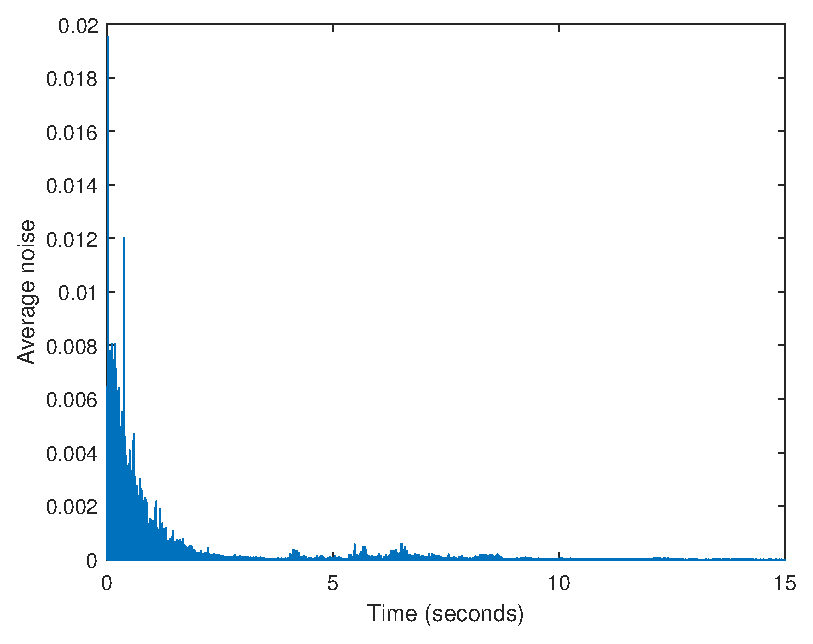
\includegraphics[width=0.5\textwidth]{figs/part1_average_noise.eps}
	\caption{Average noise averaged over 20 independent noise realizations. Note that convergence happens approximately after 4.5 seconds, which is consistent with part 1(d)}
\end{figure}

\begin{figure}[h!]
	\centering
	\begin{subfigure}[h!]{0.5\textwidth}
		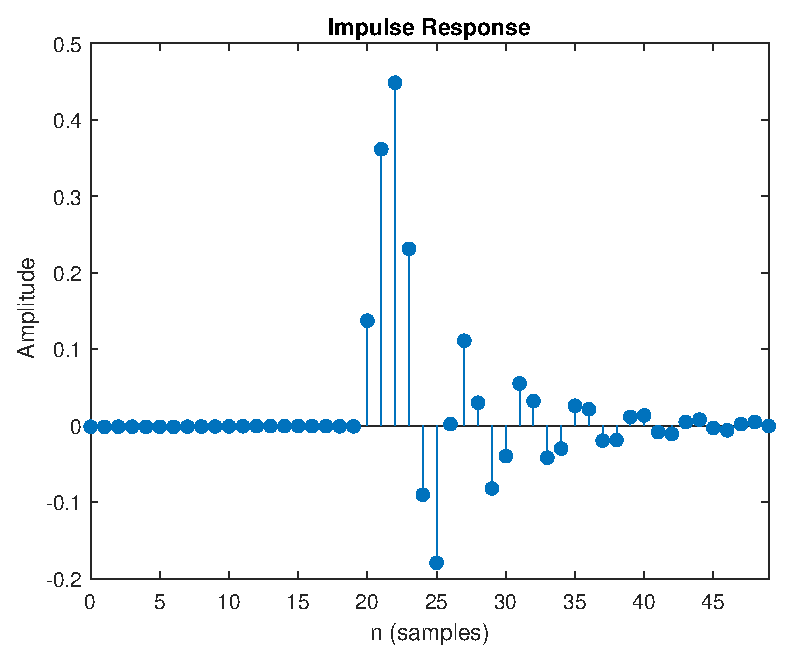
\includegraphics[width=\textwidth]{figs/part1_coeff.eps}
		\caption{Adaptive filter coefficients after adaptation.}
	\end{subfigure}%
	~ %add desired spacing between images, e. g. ~, \quad, \qquad etc.
	%(or a blank line to force the subfigure onto a new line)
	\begin{subfigure}[h!]{0.5\textwidth}
		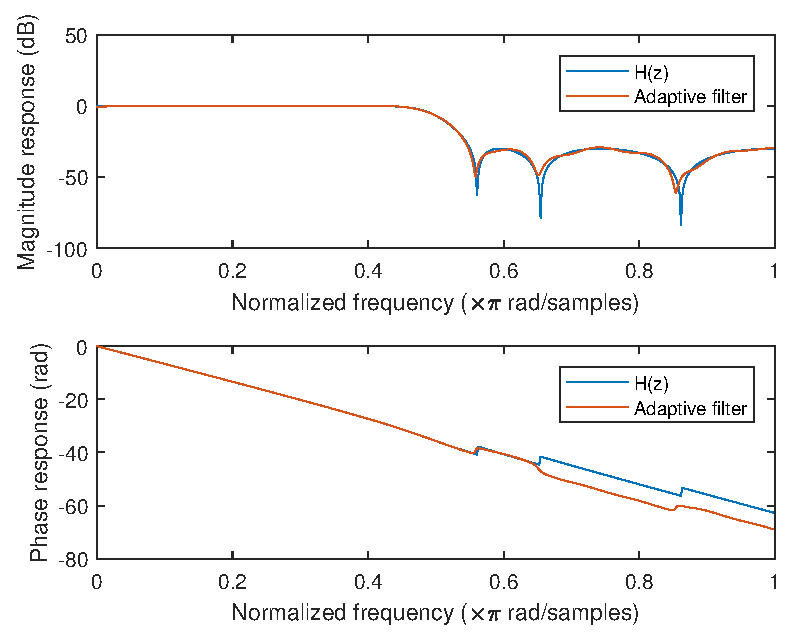
\includegraphics[width=\textwidth]{figs/part1_freqz.eps}
		\caption{Magnitude and phase response of adaptive filter after adaptation compared to $H(z)$.}
	\end{subfigure}
	\caption{Coefficients and frequency response of adaptive filter.}
\end{figure}


Ideally the adaptive filter would converge to $H(z)$. However, since $H(z)$ is IIR the adaptive FIR filter of order $L = 49$ cannot match it perfectly. Note that the first 20 coefficients of the adaptive filter are zero because of the 20-sample delay in $H(z)$.

\end{description}

\subsection{Code for part (1)}
% This file was automatically created from the m-file 
% "m2tex.m" written by USL. 
% The fontencoding in this file is UTF-8. 
%  
% You will need to include the following two packages in 
% your LaTeX-Main-File. 
%  
% \usepackage{color} 
% \usepackage{fancyvrb} 
%  
% It is advised to use the following option for Inputenc 
% \usepackage[utf8]{inputenc} 
%  
  
% definition of matlab colors: 
\definecolor{mblue}{rgb}{0,0,1} 
\definecolor{mgreen}{rgb}{0.13333,0.5451,0.13333} 
\definecolor{mred}{rgb}{0.62745,0.12549,0.94118} 
\definecolor{mgrey}{rgb}{0.5,0.5,0.5} 
\definecolor{mdarkgrey}{rgb}{0.25,0.25,0.25} 
  
\DefineShortVerb[fontfamily=courier,fontseries=m]{\$} 
\DefineShortVerb[fontfamily=courier,fontseries=b]{\#} 
  
\noindent                                                                                              
 \hspace*{-1.6em}{\scriptsize 1}$  $\color{mgrey}#%% Noise canceling#\color{black}$$\\
 \hspace*{-1.6em}{\scriptsize 2}$  clear, $\color{mdarkgrey}$clc, close all$\color{black}$$\\
 \hspace*{-1.6em}{\scriptsize 3}$   $\\
 \hspace*{-1.6em}{\scriptsize 4}$  [s, Fs] = audioread($\color{mdarkgrey}$'guitartune.wav'$\color{black}$); $\color{mgrey}$% Fs is sampling frequency$\color{black}$$\\
 \hspace*{-1.6em}{\scriptsize 5}$  $\\
 \hspace*{-1.6em}{\scriptsize 6}$  Nruns = 20; $\color{mgrey}$% number of independent runs to average learning curve$\color{black}$$\\
 \hspace*{-1.6em}{\scriptsize 7}$  var_r = 2e-3; $\color{mgrey}$% variance of white Gaussian noise$\color{black}$$\\
 \hspace*{-1.6em}{\scriptsize 8}$  $\\
 \hspace*{-1.6em}{\scriptsize 9}$  L = 49; $\color{mgrey}$% adaptive filter order. L+1 coefficients$\color{black}$$\\
 \hspace*{-2em}{\scriptsize 10}$  $\\
 \hspace*{-2em}{\scriptsize 11}$  $\color{mgrey}$% H(z) filter coefficients $\color{black}$$\\
 \hspace*{-2em}{\scriptsize 12}$  $\color{mgrey}$% Although H(z) is "unknown", for developing your answers you can use this$\color{black}$$\\
 \hspace*{-2em}{\scriptsize 13}$  $\color{mgrey}$% filter. It is a eighth-order IIR Chebyshev type II filter with bandwidth$\color{black}$$\\
 \hspace*{-2em}{\scriptsize 14}$  $\color{mgrey}$% 0.55*Fs. Chebyshev type II filters have constant gain at the passband, $\color{black}$$\\
 \hspace*{-2em}{\scriptsize 15}$  $\color{mgrey}$% but they exhibit ripples in the stopband. $\color{black}$$\\
 \hspace*{-2em}{\scriptsize 16}$  [hb, $\color{mdarkgrey}$ha] = cheby2(6, 30, 0.55);$\color{black}$$\\
 \hspace*{-2em}{\scriptsize 17}$  hb = [zeros(1, 20) hb]; $\color{mgrey}$% Add a delay of 20 samples to H(z)$\color{black}$$\\
 \hspace*{-2em}{\scriptsize 18}$  $\color{mgrey}$% Hint: for filtering, use the function filter, e.g., output = filter(hb, ha, input)$\color{black}$$\\
 \hspace*{-2em}{\scriptsize 19}$  $\\
 \hspace*{-2em}{\scriptsize 20}$  $\color{mgrey}#%% Your solutions go here#\color{black}$$\\
 \hspace*{-2em}{\scriptsize 21}$  $\color{mgrey}$% Matlab hints: $\color{black}$$\\
 \hspace*{-2em}{\scriptsize 22}$  $\color{mgrey}$% - The function randn() generates zero-mean, unit-variance,$\color{black}$$\\
 \hspace*{-2em}{\scriptsize 23}$  $\color{mgrey}$% Gaussian-distributed numbers$\color{black}$$\\
 \hspace*{-2em}{\scriptsize 24}$  $\color{mgrey}$% - Fixed filters can be easily implement using the function filter()$\color{black}$$\\
 \hspace*{-2em}{\scriptsize 25}$  $\color{mgrey}$% - Adaptive filters are can be implemented in a for loop$\color{black}$$\\
 \hspace*{-2em}{\scriptsize 26}$  $\color{mgrey}$% - To plot the coefficients of an FIR filter, use the function impz$\color{black}$$\\
 \hspace*{-2em}{\scriptsize 27}$  $\color{mgrey}$% (impulse response)$\color{black}$$\\
 \hspace*{-2em}{\scriptsize 28}$  $\color{mgrey}$% - To plot the magnitude and phase response, use the function freqz()$\color{black}$$\\
 \hspace*{-2em}{\scriptsize 29}$  $\color{mgrey}$% - To play a signal use the function sound(x, Fs). Don't forget to include$\color{black}$$\\
 \hspace*{-2em}{\scriptsize 30}$  $\color{mgrey}$% the sampling frequency when calling sound, otherwise Matlab will assume $\color{black}$$\\
 \hspace*{-2em}{\scriptsize 31}$  $\color{mgrey}$% Fs = 8 kHz, which is not the correct value.$\color{black}$$\\
 \hspace*{-2em}{\scriptsize 32}$  sound(s, $\color{mdarkgrey}$Fs) $\color{black}$$\color{mgrey}$% example$\color{black}$$\\
 \hspace*{-2em}{\scriptsize 33}$  $\\
 \hspace*{-2em}{\scriptsize 34}$  $\\
 \hspace*{-2em}{\scriptsize 35}$  $\color{mgrey}#%% Your solutions go here#\color{black}$$\\
 \hspace*{-2em}{\scriptsize 36}$  $\color{mgrey}$% (C) adaptation constant$\color{black}$$\\
 \hspace*{-2em}{\scriptsize 37}$  lamb = var_r; $\color{mgrey}$% all eigenvalues are equal to var_r since R = var_r*I$\color{black}$$\\
 \hspace*{-2em}{\scriptsize 38}$  mu = 0.001/((L+1)*var_r)$\\
 \hspace*{-2em}{\scriptsize 39}$  $\\
 \hspace*{-2em}{\scriptsize 40}$  $\color{mgrey}$% (D) convergence time$\color{black}$$\\
 \hspace*{-2em}{\scriptsize 41}$  tau = 1/(4*mu*lamb); $\color{mgrey}$% learning curve time constants$\color{black}$$\\
 \hspace*{-2em}{\scriptsize 42}$  T_conv = 4*tau/Fs $\color{mgrey}$% convergence time$\color{black}$$\\
 \hspace*{-2em}{\scriptsize 43}$  $\\
 \hspace*{-2em}{\scriptsize 44}$  $\color{mgrey}$% (F) Implementation$\color{black}$$\\
 \hspace*{-2em}{\scriptsize 45}$  $\color{mgrey}$% Generate input white noise$\color{black}$$\\
 \hspace*{-2em}{\scriptsize 46}$  r = sqrt(var_r)*randn(size(s));$\\
 \hspace*{-2em}{\scriptsize 47}$  rf = filter(hb, ha, r);$\\
 \hspace*{-2em}{\scriptsize 48}$  $\\
 \hspace*{-2em}{\scriptsize 49}$  $\color{mgrey}$% Generate signal x$\color{black}$$\\
 \hspace*{-2em}{\scriptsize 50}$  x = s + rf; $\color{mgrey}$% from diagram in Fig. 2$\color{black}$$\\
 \hspace*{-2em}{\scriptsize 51}$  $\\
 \hspace*{-2em}{\scriptsize 52}$  avg_noise = zeros(size(s));$\\
 \hspace*{-2em}{\scriptsize 53}$  $#for#$ q = 1:Nruns$\\
 \hspace*{-2em}{\scriptsize 54}$      y = zeros(size(s)); $\color{mgrey}$% output of adaptive filter$\color{black}$$\\
 \hspace*{-2em}{\scriptsize 55}$      e = zeros(size(s)); $\color{mgrey}$% error signal$\color{black}$$\\
 \hspace*{-2em}{\scriptsize 56}$      W = zeros(1, L+1); $\color{mgrey}$% initial weight vector$\color{black}$$\\
 \hspace*{-2em}{\scriptsize 57}$      $#for#$ k = L+1:length(s)$\\
 \hspace*{-2em}{\scriptsize 58}$          y(k) = W*r(k:-1:k-L);$\\
 \hspace*{-2em}{\scriptsize 59}$          e(k) = x(k) - y(k);$\\
 \hspace*{-2em}{\scriptsize 60}$          W = W + 2*mu*e(k)*r(k:-1:k-L).';$\\
 \hspace*{-2em}{\scriptsize 61}$      $#end#$$\\
 \hspace*{-2em}{\scriptsize 62}$      $\\
 \hspace*{-2em}{\scriptsize 63}$      avg_noise = avg_noise + (s-e).^2;$\\
 \hspace*{-2em}{\scriptsize 64}$  $#end#$$\\
 \hspace*{-2em}{\scriptsize 65}$  $\\
 \hspace*{-2em}{\scriptsize 66}$  avg_noise = avg_noise/Nruns;$\\
 \hspace*{-2em}{\scriptsize 67}$  $\\
 \hspace*{-2em}{\scriptsize 68}$  figure, $\color{mdarkgrey}$box on$\color{black}$$\\
 \hspace*{-2em}{\scriptsize 69}$  plot((0:length(s)-1)/Fs, $\color{mdarkgrey}$avg_noise)$\color{black}$$\\
 \hspace*{-2em}{\scriptsize 70}$  xlabel($\color{mdarkgrey}$'Time (seconds)'$\color{black}$)$\\
 \hspace*{-2em}{\scriptsize 71}$  ylabel($\color{mdarkgrey}$'Average noise'$\color{black}$)$\\
 \hspace*{-2em}{\scriptsize 72}$  saveas(gca, $\color{mdarkgrey}$'../figs/part1_average_noise'$\color{black}$, $\color{mdarkgrey}$'epsc'$\color{black}$)$\\
 \hspace*{-2em}{\scriptsize 73}$  $\\
 \hspace*{-2em}{\scriptsize 74}$  figure, $\color{mdarkgrey}$impz(W)$\color{black}$$\\
 \hspace*{-2em}{\scriptsize 75}$  saveas(gca, $\color{mdarkgrey}$'../figs/part1_coeff'$\color{black}$, $\color{mdarkgrey}$'epsc'$\color{black}$)$\\
 \hspace*{-2em}{\scriptsize 76}$  $\\
 \hspace*{-2em}{\scriptsize 77}$  [H1, $\color{mdarkgrey}$w] = freqz(hb, ha);$\color{black}$$\\
 \hspace*{-2em}{\scriptsize 78}$  H2 = freqz(W, 1, w);$\\
 \hspace*{-2em}{\scriptsize 79}$  $\\
 \hspace*{-2em}{\scriptsize 80}$  figure$\\
 \hspace*{-2em}{\scriptsize 81}$  subplot(211), $\color{mdarkgrey}$hold on, box on$\color{black}$$\\
 \hspace*{-2em}{\scriptsize 82}$  plot(w/pi, $\color{mdarkgrey}$20*log10(abs(H1)))$\color{black}$$\\
 \hspace*{-2em}{\scriptsize 83}$  plot(w/pi, $\color{mdarkgrey}$20*log10(abs(H2)))$\color{black}$$\\
 \hspace*{-2em}{\scriptsize 84}$  xlabel($\color{mdarkgrey}$'Normalized frequency (\times\pi rad/samples)'$\color{black}$)$\\
 \hspace*{-2em}{\scriptsize 85}$  ylabel($\color{mdarkgrey}$'Magnitude response (dB)'$\color{black}$)$\\
 \hspace*{-2em}{\scriptsize 86}$  legend($\color{mdarkgrey}$'H(z)'$\color{black}$, $\color{mdarkgrey}$'Adaptive filter'$\color{black}$)$\\
 \hspace*{-2em}{\scriptsize 87}$  $\\
 \hspace*{-2em}{\scriptsize 88}$  subplot(212), $\color{mdarkgrey}$hold on, box on$\color{black}$$\\
 \hspace*{-2em}{\scriptsize 89}$  plot(w/pi, $\color{mdarkgrey}$unwrap(angle(H1)))$\color{black}$$\\
 \hspace*{-2em}{\scriptsize 90}$  plot(w/pi, $\color{mdarkgrey}$unwrap(angle(H2)))$\color{black}$$\\
 \hspace*{-2em}{\scriptsize 91}$  xlabel($\color{mdarkgrey}$'Normalized frequency (\times\pi rad/samples)'$\color{black}$)$\\
 \hspace*{-2em}{\scriptsize 92}$  ylabel($\color{mdarkgrey}$'Phase response (rad)'$\color{black}$)$\\
 \hspace*{-2em}{\scriptsize 93}$  legend($\color{mdarkgrey}$'H(z)'$\color{black}$, $\color{mdarkgrey}$'Adaptive filter'$\color{black}$)$\\
 \hspace*{-2em}{\scriptsize 94}$  saveas(gca, $\color{mdarkgrey}$'../figs/part1_freqz'$\color{black}$, $\color{mdarkgrey}$'epsc'$\color{black}$)$\\ 
  
\UndefineShortVerb{\$} 
\UndefineShortVerb{\#}

\section{Problem 2}

\begin{description}
	\item[(a)] The DFT of a constant signal is an impulse scaled by the d.c. value: 
	\begin{equation}
		X[k] = \{8, 0, 0, 0, 0, 0, 0, 0\}
	\end{equation}
	
	\item[(b)] This signal can be represented as  $x[n] = e^{j\pi n}, n = 0, \ldots, 7$. Start with the result from part (a) and use the circular time shift property of the DFT. Note that for $N = 8$, 
	
	\begin{equation}
	(-1) = e^{j\pi n} = W_N^{-N/2n}
	\end{equation}
	Using the circular frequency shift property, the DFT is a shift of the DFT from part (a) by $N/2 = 4$: $X[k] = \{0, 0, 0, 0, 8, 0, 0, 0\}$
	
	\item[(c)] This is similar to part (b). Note that for $N = 8$
	\begin{equation}
	e^{j\pi/2n} = e^{j2\pi/N N/4n} = W_N^{-N/4n}.
	\end{equation}
	Using the circular frequency shift property, the DFT is a shift of the DFT from part (a) by $N/4 = 2$: $X[k] = \{0, 0, 8, 0, 0, 0, 0, 0\}$
	
	\item[(d)] Start withe the result of part (c). Note that $sin(\pi n/2) = -j/2(e^{j\pi n/2} - e^{-j\pi n/2})$. Using the circular frequency shift property, we find that $X[k] = \{0, 0, -4j, 0, 0, 0, 4j, 0\}$
	
	\item[(e)] The DFT of an impulse is constant in frequency: $X[k] = \{1, 1, 1, 1, 1, 1, 1, 1\}$.
	
	\item[(f)] Circularly shifting a signal in time corresponds to multiplication by a complex exponential in frequency. Using part (e), we find that: $X[k] = \{1, -j, -1, j, 1, -j, -1, j\}$.  
\end{description}

\section{Problem 3}	
	\begin{center}
		\begin{tabular}{c|c|p{10cm}}
			Signal & DFT & Justification \\
			\hline
			1 & d & $x[n]$ is real and $x[n] = x[((-n))_N]$ ($\tilde{x}[n]$ is even), so $X[k]$ is purely real, thus $\angle X[k] \in \{0, \pi\}$. Also, $\sum_{n =0}^{N-1}x[n] = X[0] = 5$. \\
			\hline
			2 & a & $x[n]$ is real and $x[n] = x[((-n))_N]$ ($\tilde{x}[n]$ is even), so $X[k]$ is purely real, thus $\angle X[k] \in \{0, \pi\}$. Also, $\sum_{n =0}^{N-1}x[n] = X[0] = 1$. \\
			\hline
			3 & c & $x[n]$ is real and $x[n] = -x[((-n))_N]$ ($\tilde{x}[n]$ is odd), so $X[k]$ is purely imaginary, thus $\angle X[k] \in \{-\pi/2, \pi/2\}$. Also, $\sum_{n =0}^{N-1}x[n] = X[0] = 0$. \\
			\hline
			4 & f & $x[n]$ is delayed impulse, so $|X[k]| = 1~\forall~k$ \\
			\hline
			5 & b & Signal 5 is a delayed version of signal 1, so $|X[k]|$ same as for signal 1. But signal 5 lacks symmetry, so $\angle X[k]$ is more complicated than for signal 1.\\
			\hline
			6 & e & Signal 6 is a delayed version of signal 3, so $|X[k]|$ same as for signal 3. But signal 6 lacks symmetry, so $\angle X[k]$ is more complicated than for signal 3. \\
			\hline
		\end{tabular}
	\end{center}


\section{Problem 4: Linear convolution and circular convolution}	
\subsection{(a)}
We will have $x[n]\ast h[n] = x[n]~\encircle{N}~h[n]$ as long as
\begin{equation}
	N \geq L + P - 1
\end{equation}
\subsection{(b)}

\begin{align*}
	c_{xy}[m] &= x[m] \ast y^*[-m] \\
	&= x[m]~\encircle{N}~y^*[-m] \tag{as long as $N \geq 2L - 1$} \\
	&= \mathrm{IFFT}\{\mathrm{FFT}\{x[m]\}(\mathrm{FFT}\{y[m]\})^*\} ,
\end{align*}
where the last equality follows since circular convolution in time domain corresponds to product of DFTs in frequency domain. Moreover, we've used the conjugate and time reversal properties of the DFT i.e., $\mathrm{FFT}\{y^*[-m]\} = (\mathrm{FFT}\{y[m]\})^*$. The FFT/IFFT involved in this calculation are $N = 2L-1$.

As mentioned in the hint, this computation will provide $c_{xy}[m]$ indexed from $0$ up to $N-1$. We would need to use the function \texttt{fftshfit}, for instance, to produce $c_{xy}[m]$ in the conventional representation from $-N/2+1$ up to $N/2-1$.

\subsection{(c)}

If $x[n] = y[n]$, then 

\begin{align}
c_{xx}[m] = \mathrm{IFFT}\{|\mathrm{FFT}\{x[m]\}|^2\}
\end{align}
Hence this computation requires one fewer FFT.

\section{Problem 5: Overlap-add or overlap-save}	
\subsection{(a)}

The code for for part (a) is attached at the end of this question. The implementation assumes FFT length $N = 256$, and $M = 52$.

The Figures below show the results of comparison for overlap-add and overlap-save methods. We obtain the same results as with direct implementation of the FIR filter. The disagreement at the end of the sequence is simply because we did not have an entire block to perform block convolution. 

\FloatBarrier
\begin{figure}[h!]
	\centering
	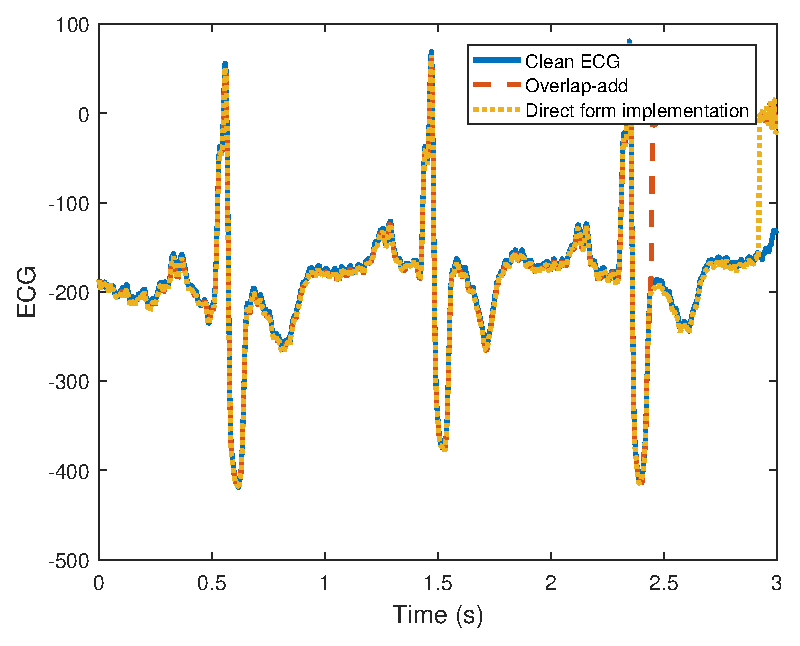
\includegraphics[scale=0.8]{fir_notch_overlap_add.eps}
	\caption{Result using the overlap-add method}
\end{figure}
\FloatBarrier

\FloatBarrier
\begin{figure}[h!]
	\centering
	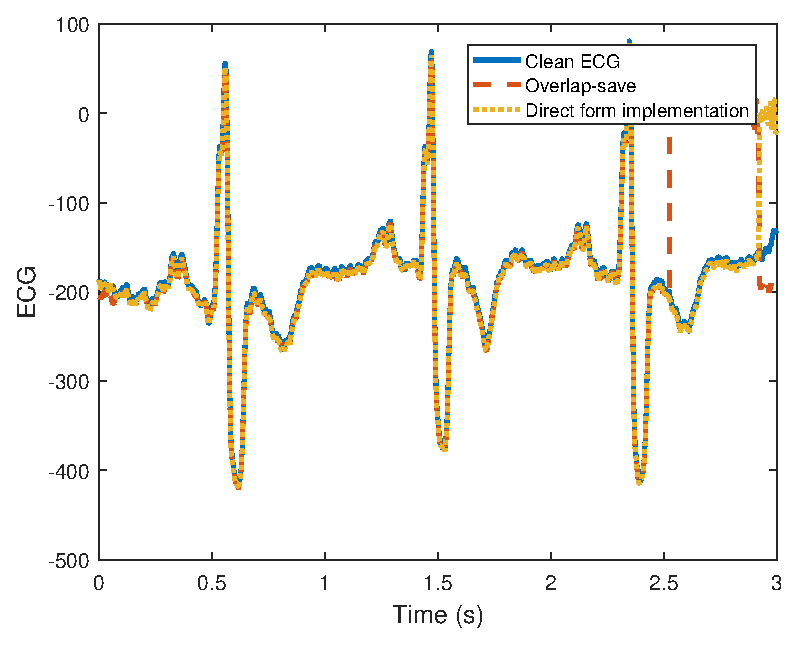
\includegraphics[scale=0.8]{fir_notch_overlap_save.eps}
	\caption{Result using the overlap-save method.}
\end{figure}
\FloatBarrier

\subsection{(b)}

Without any simplification, the block convolution requires 3 FFTs (including IFFT) are necessary to produce $N-M$ useful output samples. Therefore,

\begin{equation}
	C = \frac{(3\times (2N(\log_2(N)-1)) + N)}{N-M} = 53.4369 \tag{block convolution}
\end{equation}
for $N = 256$ and $M = 52$.

The direct form implementation of a $M$th-order FIR filter (without any symmetry) requires $M+1$ multiplications per useful output. Thus,

\begin{equation}
C = M+1 = 53 \tag{FIR direct implementation}
\end{equation}

\noindent\textbf{Simplifications:}

Note that the FFT to compute the filter coefficients may be computed in advance and stored in a memory since the filter is assumed constant. Thus, we could avoid 1 FFT:
\begin{equation}
C = \frac{(2\times (2N(\log_2(N)-1)) + N)}{N-M} = 36.038 \tag{block convolution}
\end{equation}
assuming $N = 256$ and $M = 52$.

An linear phase FIR filter requires $\lfloor (M+1)/2 \rfloor$ multiplications per useful output, since equal coefficients can be combined. Therefore, 
\begin{equation}
C = \lfloor (M+1)/2 \rfloor =  26 \tag{linear phase FIR direct implementation}
\end{equation}
For $M = 52$.

Solutions with or without these simplifications are accepted.

\subsection{(c)}
For both overlap-add and overlap-save methods, we need 3 FFTs (including IFFT), and an $N$-point multiplication. Moreover, for each block of length $L$ only $N - M$ outputs are useful. In the overlap-save method there are $M$ unusable outputs per block. In the overlap-add method the $M$ outputs will only be useful at the next block.

\begin{align}
C = \frac{3\times (2N(\log_2(N)-1)) + N}{N-M} \tag{block convolution}
\end{align}

Assuming that the DFT of the filter coefficients is computed in advance:
\begin{equation}
C = \frac{2\times (2N(\log_2(N)-1)) + N}{N-M} \tag{block convolution 2 FFTs}
\end{equation}

Both results for $C$ are accepted. The figure below assumes that $C$ was computed in accordance with the equation above, assuming that the DFT of the filter coefficients was computed in advance:

\FloatBarrier
\begin{figure}[h!]
	\centering
	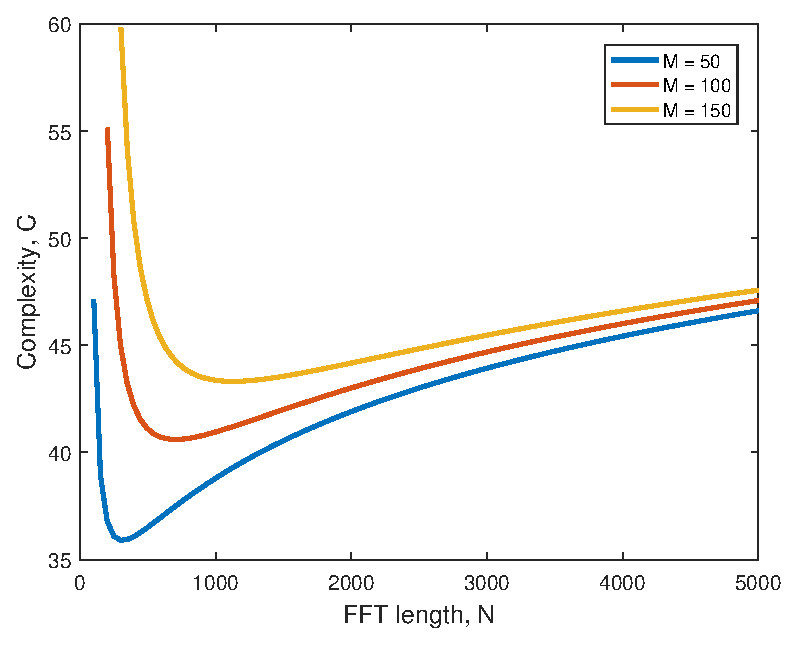
\includegraphics[scale=0.8]{block_conv_complexity.eps}
	\caption{Complexity of overlap-save or overlap-add method as a function of the FFT length. These curves assumed that the DFT of the filter coefficients was computed in advance, hence saving one FFT in the complexity calculations.}
\end{figure}
\FloatBarrier

Note that for each filter length there is an optimal FFT length. 

Moreover, note that as the filter-order becomes large, the FFT implementation becomes more attractive even if we assume that there's symmetry in the impulse response of the filter. For $M = 100$, the block convolution method has complexity close to $C =40$, while a direct implementation assuming symmetry would have complexity $C = 50$.


\noindent\textbf{Note:} the particular formula for the number of real multiplications of $N$-point FFT considered in this problem is only valid when $N$ is a power of 2. The actual number of multiplications in a FFT depend on whether the FFT is radix-2, radix-4, prime radix, etc. The actual values will vary slightly, but the main conclusions from this problem remain the same. 

\subsection{(d) (optional)}

See Matlab code below for solution. Plots are shown in part (a).

\subsection{Matlab code for Problem 4}
% This file was automatically created from the m-file 
% "m2tex.m" written by USL. 
% The fontencoding in this file is UTF-8. 
%  
% You will need to include the following two packages in 
% your LaTeX-Main-File. 
%  
% \usepackage{color} 
% \usepackage{fancyvrb} 
%  
% It is advised to use the following option for Inputenc 
% \usepackage[utf8]{inputenc} 
%  
  
% definition of matlab colors: 
\definecolor{mblue}{rgb}{0,0,1} 
\definecolor{mgreen}{rgb}{0.13333,0.5451,0.13333} 
\definecolor{mred}{rgb}{0.62745,0.12549,0.94118} 
\definecolor{mgrey}{rgb}{0.5,0.5,0.5} 
\definecolor{mdarkgrey}{rgb}{0.25,0.25,0.25} 
  
\DefineShortVerb[fontfamily=courier,fontseries=m]{\$} 
\DefineShortVerb[fontfamily=courier,fontseries=b]{\#} 
  
\noindent                                                                         
 \hspace*{-1.6em}{\scriptsize 1}$  $\color{mgrey}#%% Overlap and save or overlap and add#\color{black}$$\\
 \hspace*{-1.6em}{\scriptsize 2}$  clear, $\color{mdarkgrey}$clc, close all$\color{black}$$\\
 \hspace*{-1.6em}{\scriptsize 3}$  $\\
 \hspace*{-1.6em}{\scriptsize 4}$  load($\color{mdarkgrey}$'notch_filter_coeff'$\color{black}$); $\color{mgrey}$% loads filter coefficients$\color{black}$$\\
 \hspace*{-1.6em}{\scriptsize 5}$  load($\color{mdarkgrey}$'ecg_recording.mat'$\color{black}$)  $\color{mgrey}$% loads ECG data$\color{black}$$\\
 \hspace*{-1.6em}{\scriptsize 6}$  $\\
 \hspace*{-1.6em}{\scriptsize 7}$  $\color{mgrey}$% Definitions$\color{black}$$\\
 \hspace*{-1.6em}{\scriptsize 8}$  Nfft = 256;    $\color{mgrey}$% FFT length$\color{black}$$\\
 \hspace*{-1.6em}{\scriptsize 9}$  M = length(hls) - 1; $\color{mgrey}$% M = 52$\color{black}$$\\
 \hspace*{-2em}{\scriptsize 10}$  Loa = Nfft - M; $\color{mgrey}$% block length for overlap-add$\color{black}$$\\
 \hspace*{-2em}{\scriptsize 11}$  Los = Nfft;     $\color{mgrey}$% block length for overlap-save$\color{black}$$\\
 \hspace*{-2em}{\scriptsize 12}$  H = fft(hls, Nfft); $\color{mgrey}$% FFT of filter coefficients$\color{black}$$\\
 \hspace*{-2em}{\scriptsize 13}$  $\\
 \hspace*{-2em}{\scriptsize 14}$  t = 0:T:(N-1)*T; $\color{mgrey}$% time vector$\color{black}$$\\
 \hspace*{-2em}{\scriptsize 15}$  ecg_fir = filter(hls, 1, ecg_60Hz);$\\
 \hspace*{-2em}{\scriptsize 16}$  ecg_fir = circshift(ecg_fir, [0, -M/2]); $\color{mgrey}$% remove group delay$\color{black}$$\\
 \hspace*{-2em}{\scriptsize 17}$  $\\
 \hspace*{-2em}{\scriptsize 18}$  $\color{mgrey}#%% Overlap-add#\color{black}$$\\
 \hspace*{-2em}{\scriptsize 19}$  yoa = zeros(size(ecg_60Hz));$\\
 \hspace*{-2em}{\scriptsize 20}$  select = (1:Loa);$\\
 \hspace*{-2em}{\scriptsize 21}$  $#for#$ r = 0:floor(length(ecg_60Hz)/Loa)-1$\\
 \hspace*{-2em}{\scriptsize 22}$      xr = ecg_60Hz(select);           $\color{mgrey}$% non-overlapping segments of length Loa$\color{black}$$\\
 \hspace*{-2em}{\scriptsize 23}$      yr = ifft(H.*fft(xr, Nfft));    $\color{mgrey}$% compute Nfft-point circular convolution$\color{black}$$\\
 \hspace*{-2em}{\scriptsize 24}$      yoa(select(1):(select(1)+Nfft-1)) = yoa(select(1):(select(1)+Nfft-1)) + yr; $\color{mgrey}$% add$\color{black}$$\\
 \hspace*{-2em}{\scriptsize 25}$      select = select + Loa;$\\
 \hspace*{-2em}{\scriptsize 26}$  $#end#$$\\
 \hspace*{-2em}{\scriptsize 27}$  $\\
 \hspace*{-2em}{\scriptsize 28}$  figure, $\color{mdarkgrey}$hold on, box on$\color{black}$$\\
 \hspace*{-2em}{\scriptsize 29}$  n = 0:length(ecg_60Hz)-1;$\\
 \hspace*{-2em}{\scriptsize 30}$  yoa = circshift(yoa, [0, -M/2]); $\color{mgrey}$% remove group delay$\color{black}$$\\
 \hspace*{-2em}{\scriptsize 31}$  plot(t, ecg_clean, $\color{mdarkgrey}$'LineWidth'$\color{black}$, 2, $\color{mdarkgrey}$'DisplayName'$\color{black}$, $\color{mdarkgrey}$'Clean ECG'$\color{black}$)$\\
 \hspace*{-2em}{\scriptsize 32}$  plot(t, yoa, $\color{mdarkgrey}$'--'$\color{black}$, $\color{mdarkgrey}$'LineWidth'$\color{black}$, 2, $\color{mdarkgrey}$'displayname'$\color{black}$, $\color{mdarkgrey}$'Overlap-add'$\color{black}$)$\\
 \hspace*{-2em}{\scriptsize 33}$  plot(t, ecg_fir, $\color{mdarkgrey}$':'$\color{black}$, $\color{mdarkgrey}$'LineWidth'$\color{black}$, 2, $\color{mdarkgrey}$'displayname'$\color{black}$, $\color{mdarkgrey}$'Direct form implementation'$\color{black}$)$\\
 \hspace*{-2em}{\scriptsize 34}$  legend($\color{mdarkgrey}$'-dynamiclegend'$\color{black}$)$\\
 \hspace*{-2em}{\scriptsize 35}$  xlabel($\color{mdarkgrey}$'Time (s)'$\color{black}$, $\color{mdarkgrey}$'FontSize'$\color{black}$, 12)$\\
 \hspace*{-2em}{\scriptsize 36}$  ylabel($\color{mdarkgrey}$'ECG'$\color{black}$, $\color{mdarkgrey}$'FontSize'$\color{black}$, 12)$\\
 \hspace*{-2em}{\scriptsize 37}$  saveas(gca, $\color{mdarkgrey}$'../figs/fir_notch_overlap_add'$\color{black}$, $\color{mdarkgrey}$'epsc'$\color{black}$)$\\
 \hspace*{-2em}{\scriptsize 38}$  $\\
 \hspace*{-2em}{\scriptsize 39}$  $\color{mgrey}#%% Overlap-save#\color{black}$$\\
 \hspace*{-2em}{\scriptsize 40}$  yos = zeros(size(ecg_60Hz));$\\
 \hspace*{-2em}{\scriptsize 41}$  select = (1:Los);$\\
 \hspace*{-2em}{\scriptsize 42}$  $#for#$ r = 0:floor(length(ecg_60Hz)/Los)$\\
 \hspace*{-2em}{\scriptsize 43}$      xr = ecg_60Hz(select);           $\color{mgrey}$% non-overlapping segments of length Loa$\color{black}$$\\
 \hspace*{-2em}{\scriptsize 44}$      yr = ifft(H.*fft(xr, Nfft));    $\color{mgrey}$% compute Nfft-point circular convolution$\color{black}$$\\
 \hspace*{-2em}{\scriptsize 45}$      yoa(select(M+1:end)) = yr(M+1:end); $\color{mgrey}$% save$\color{black}$$\\
 \hspace*{-2em}{\scriptsize 46}$      select = select + Los - M;$\\
 \hspace*{-2em}{\scriptsize 47}$  $#end#$$\\
 \hspace*{-2em}{\scriptsize 48}$  $\\
 \hspace*{-2em}{\scriptsize 49}$  figure, $\color{mdarkgrey}$hold on, box on$\color{black}$$\\
 \hspace*{-2em}{\scriptsize 50}$  n = 0:length(ecg_60Hz)-1;$\\
 \hspace*{-2em}{\scriptsize 51}$  yoa = circshift(yoa, [0, -M/2]); $\color{mgrey}$% remove group delay$\color{black}$$\\
 \hspace*{-2em}{\scriptsize 52}$  plot(t, ecg_clean, $\color{mdarkgrey}$'LineWidth'$\color{black}$, 2, $\color{mdarkgrey}$'DisplayName'$\color{black}$, $\color{mdarkgrey}$'Clean ECG'$\color{black}$)$\\
 \hspace*{-2em}{\scriptsize 53}$  plot(t, yoa, $\color{mdarkgrey}$'--'$\color{black}$, $\color{mdarkgrey}$'LineWidth'$\color{black}$, 2, $\color{mdarkgrey}$'displayname'$\color{black}$, $\color{mdarkgrey}$'Overlap-save'$\color{black}$)$\\
 \hspace*{-2em}{\scriptsize 54}$  plot(t, ecg_fir, $\color{mdarkgrey}$':'$\color{black}$, $\color{mdarkgrey}$'LineWidth'$\color{black}$, 2, $\color{mdarkgrey}$'displayname'$\color{black}$, $\color{mdarkgrey}$'Direct form implementation'$\color{black}$)$\\
 \hspace*{-2em}{\scriptsize 55}$  legend($\color{mdarkgrey}$'-dynamiclegend'$\color{black}$)$\\
 \hspace*{-2em}{\scriptsize 56}$  xlabel($\color{mdarkgrey}$'Time (s)'$\color{black}$, $\color{mdarkgrey}$'FontSize'$\color{black}$, 12)$\\
 \hspace*{-2em}{\scriptsize 57}$  ylabel($\color{mdarkgrey}$'ECG'$\color{black}$, $\color{mdarkgrey}$'FontSize'$\color{black}$, 12)$\\
 \hspace*{-2em}{\scriptsize 58}$  saveas(gca, $\color{mdarkgrey}$'../figs/fir_notch_overlap_save'$\color{black}$, $\color{mdarkgrey}$'epsc'$\color{black}$)$\\
 \hspace*{-2em}{\scriptsize 59}$  $\\
 \hspace*{-2em}{\scriptsize 60}$  $\color{mgrey}#%% Complexity calculation#\color{black}$$\\
 \hspace*{-2em}{\scriptsize 61}$  M = 50:50:150;$\\
 \hspace*{-2em}{\scriptsize 62}$  $\\
 \hspace*{-2em}{\scriptsize 63}$  C = @(N, M) (2*2*N.*(log2(N)-1) + N)./(N-M);$\\
 \hspace*{-2em}{\scriptsize 64}$  $\\
 \hspace*{-2em}{\scriptsize 65}$  figure, $\color{mdarkgrey}$hold on, box on$\color{black}$$\\
 \hspace*{-2em}{\scriptsize 66}$  $#for#$ k = 1:length(M)$\\
 \hspace*{-2em}{\scriptsize 67}$      N = linspace(M(k)*2, 5e3);$\\
 \hspace*{-2em}{\scriptsize 68}$      plot(N, C(N, M(k)), $\color{mdarkgrey}$'LineWidth'$\color{black}$, 2, $\color{mdarkgrey}$'DisplayName'$\color{black}$, sprintf($\color{mdarkgrey}$'M = %d'$\color{black}$, M(k)))$\\
 \hspace*{-2em}{\scriptsize 69}$  $#end#$$\\
 \hspace*{-2em}{\scriptsize 70}$  xlabel($\color{mdarkgrey}$'FFT length'$\color{black}$, $\color{mdarkgrey}$'FontSize'$\color{black}$, 12)$\\
 \hspace*{-2em}{\scriptsize 71}$  ylabel($\color{mdarkgrey}$'Complexity'$\color{black}$, $\color{mdarkgrey}$'FontSize'$\color{black}$, 12)$\\
 \hspace*{-2em}{\scriptsize 72}$  legend($\color{mdarkgrey}$'-dynamiclegend'$\color{black}$)$\\
 \hspace*{-2em}{\scriptsize 73}$  saveas(gca, $\color{mdarkgrey}$'../figs/block_conv_complexity'$\color{black}$, $\color{mdarkgrey}$'epsc'$\color{black}$)$\\ 
  
\UndefineShortVerb{\$} 
\UndefineShortVerb{\#}


\section{Problem 6: Spectrograms}
\begin{description}
	\item[(a)] Spectrograms (a) and (c) were computed with the rectangular window. This can be infered from the amount of leakage in the spectrogram. This is a result from the large sidelobes of the rectangular window.
	\item[(b)] Spectrograms (a) \& (b) have approximately the same frequency resolution, as do spectrograms (c) \& (d). Note that the the lines in these spectrograms have approximately the same thickness
	\item[(c)] Spectrogram (c) has the shortest time window. Although spectrograms (c) and (d) have virtually the same frequency resolution i.e., same main-lobe width, the Hamming window has to be longer to achieve the same main-lobe width of a rectangular window. This is the reason that, for instance, a filter designed by window using the Hamming window would have slower roll-off than a filter designed using a rectangular window of same length.
	\item[(d)] 
	The discrete-time signal has three frequency components
	\begin{equation}
		x[n] = \begin{cases}
		A_1\cos(0.7\pi n + \phi_1) + A_2\cos(0.4\pi n + \phi_2), & 0 \leq n \leq 1000 \\
		A_2\cos(0.4\pi n + \phi_2), & 1000 < n \leq 2000 \\
		A_2\cos(0.4\pi n + \phi_2) + A_3\cos(0.5\pi n + \phi_3), & 2000 < n \leq 3000 \\
		\end{cases}
	\end{equation}
	We cannot specify the amplitudes $\{A_1, A_2, A_3\}$ and the phases $\{\phi_1, \phi_2, \phi_3\}$.
	
	To obtain the continuous-time signal, we simply replace $n$ by $t/T$
	\begin{equation}
		x_c(t) = \begin{cases}
		A_1\cos(7000\pi t + \phi_1) + A_2\cos(4000\pi t + \phi_2), & 0 \leq n \leq 1000 \\
		A_2\cos(4000\pi t + \phi_2), & 1000 < n \leq 2000 \\
		A_2\cos(4000\pi t + \phi_2) + A_3\cos(5000\pi t + \phi_3), & 2000 < n \leq 3000 \\
		\end{cases}
	\end{equation}
	
	Note that the anplitudes should be scaled by $T$, but we simply redefined the amplitudes for simplicity. 
	
\end{description}

\section{Problem 7: Frequency modulation}

\subsection{(a)}

\begin{equation}
	\Omega_i(t) = \dfrac{d\theta(t)}{dt} = \Omega_c + \beta\Omega_m\cos(\Omega_mt)
\end{equation}

Hence, the maximum frequency deviation from $\Omega_c$ is $\beta\Omega_m$.

\FloatBarrier
\begin{figure}[h!]
	\centering
	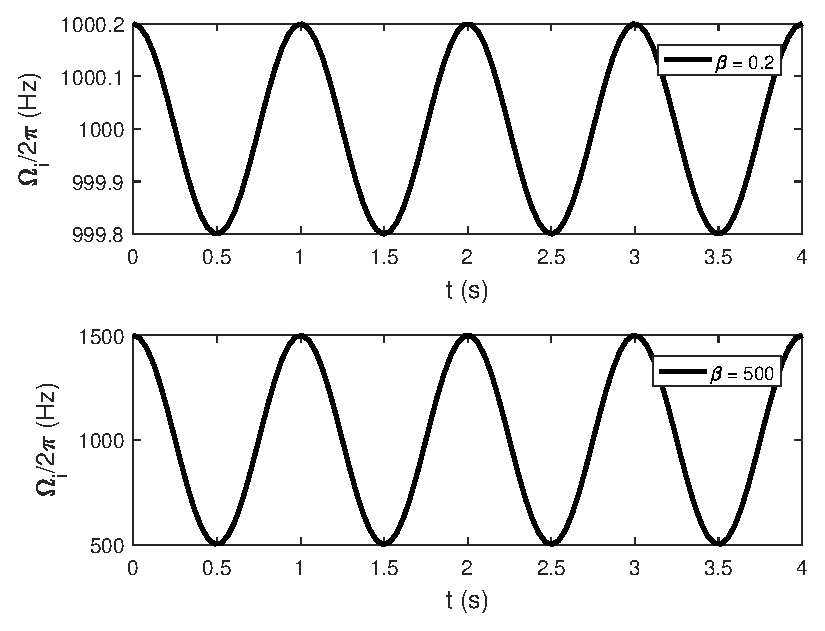
\includegraphics[scale=0.8]{hw6_fm_a.eps}
	\caption{$\Omega_i(t)/(2\pi)$ for $\beta = 0.2$ (top) and $\beta = 500$ (bottom).}
\end{figure}
\FloatBarrier

\subsection{(b)}

\begin{align} \nonumber \label{xfmapprox}
	x_{FM}(t) &= \cos(\Omega_ct + \beta\sin(\Omega_m t)) \\ \nonumber
	&= \cos(\Omega_ct)\cos(\beta\sin(\Omega_m t)) - \sin(\Omega_ct)\sin(\beta\sin(\Omega_m t)) \\ 
	& \approx \cos(\Omega_ct) - \beta\sin(\Omega_m t)\sin(\Omega_ct) \tag{small-angle approximation when $\beta << \pi/2$}
\end{align}

By inspecting the equation above, we can see that $\mathcal{F}\{x_{FM}(t)\}$ has impulses at frequencies $\pm\Omega_c$, $\pm\Omega_c + \Omega_m$, and $\pm\Omega_c - \Omega_m$.

\subsection{(c)}

We simply replace $t = nT$ in (3) of the assignment, 
\begin{align} \nonumber
	x_{FM}[n] &= x_{FM}(nT) = \cos(2\pi(1000) n/8000 + \beta\sin(2\pi n/8000)) \\
	&\cos(\pi/4 n + \beta\sin(\pi n/4000))
\end{align}

\subsection{(d)}
Code for this part is attached at the end of this problem

\subsubsection{(i)}
\FloatBarrier
\begin{figure}[h!]
	\centering
	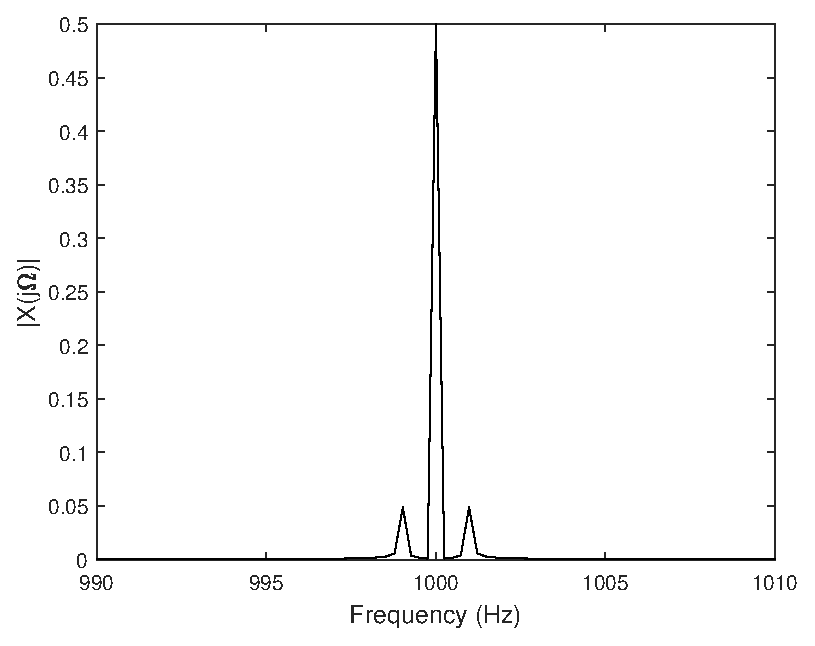
\includegraphics[scale=0.7]{figs/hw6_fm_di.eps}
	\caption{DFT of $x_{FM}(t)$ for $\beta = 0.2$.}
\end{figure}
\FloatBarrier

\subsubsection{(ii)}
\FloatBarrier
\begin{figure}[h!]
	\centering
	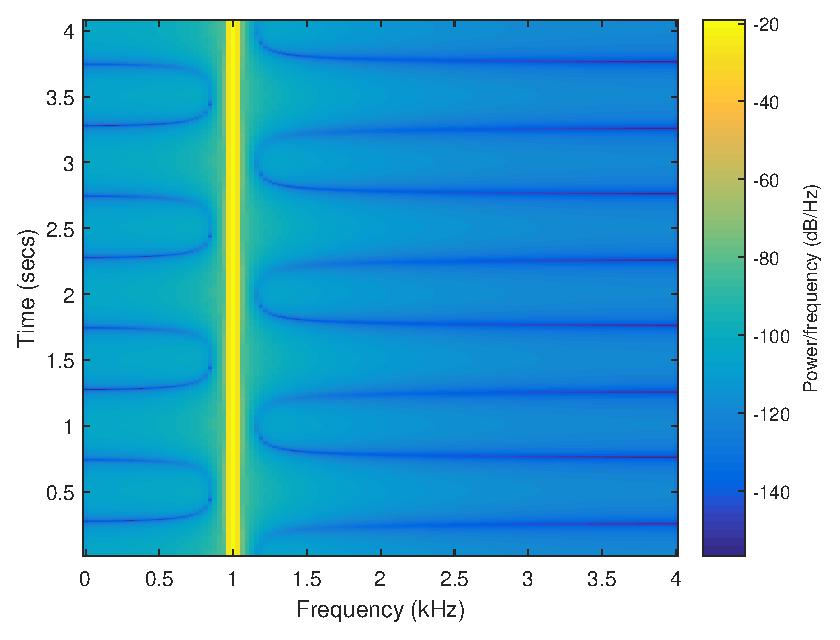
\includegraphics[scale=0.7]{figs/hw6_fm_dii.eps}
	\caption{Spectrogram of $x_{FM}(t)$ for $\beta = 0.2$.}
\end{figure}
\FloatBarrier

The spectrogram does not show the frequency variation observed in part (a) because the window does not have enough resolution to resolve the frequency variation when $\beta = 0.2$.


\subsection{(e)}
Code for this part is attached at the end of this problem

\subsubsection{(i)}
\FloatBarrier
\begin{figure}[h!]
	\centering
	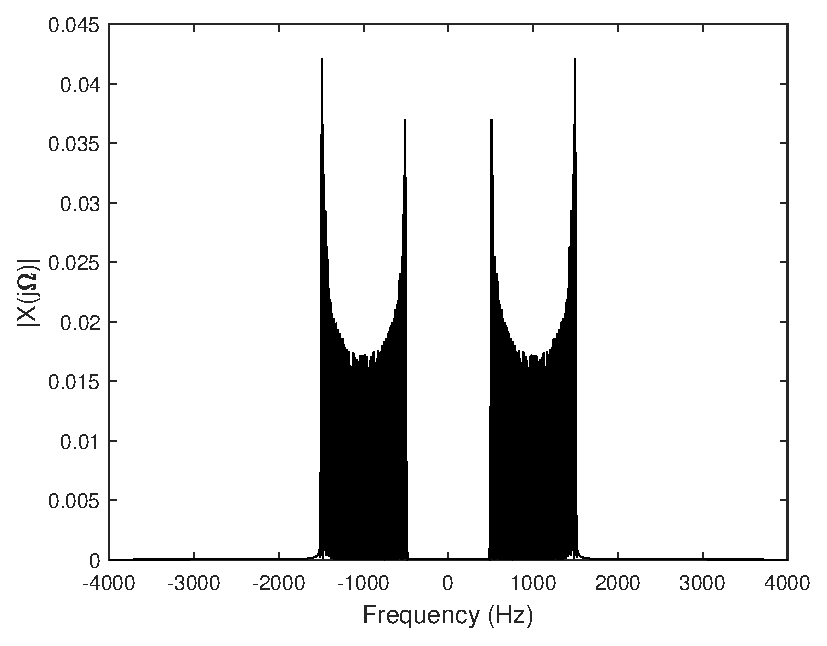
\includegraphics[scale=0.7]{figs/hw6_fm_ei.eps}
	\caption{DFT of $x_{FM}(t)$ for $\beta = 500$.}
\end{figure}
\FloatBarrier

\subsubsection{(ii)}
\FloatBarrier
\begin{figure}[h!]
	\centering
	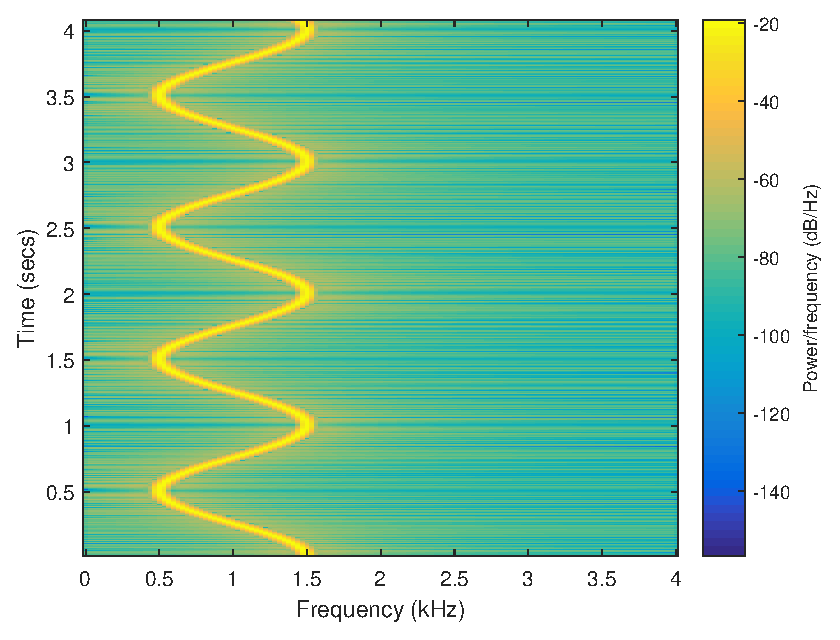
\includegraphics[scale=0.7]{figs/hw6_fm_eii.eps}
	\caption{Spectrogram of $x_{FM}(t)$ for $\beta = 500$.}
\end{figure}
\FloatBarrier

Now the frequency variation is large enough that we can observe it in the spectrogram. 

\subsubsection{(iii)}

Increasing the window length improves frequency resolution. However, by making the window length too large may lead to excessive leakage, since the sidelobes area may become significant.

If $\Omega_m$ is small, we must make the window longer in order to improve the frequency resolution. 

The window length does not depend on $\Omega_c$ provided that the frequency variations $\Omega_c + \beta\Omega_m$ does not cause aliasing. That is, $\Omega_c + \beta\Omega_m < \Omega_s/2$.

\subsection{Code for Problem 6}
% This file was automatically created from the m-file 
% "m2tex.m" written by USL. 
% The fontencoding in this file is UTF-8. 
%  
% You will need to include the following two packages in 
% your LaTeX-Main-File. 
%  
% \usepackage{color} 
% \usepackage{fancyvrb} 
%  
% It is advised to use the following option for Inputenc 
% \usepackage[utf8]{inputenc} 
%  
  
% definition of matlab colors: 
\definecolor{mblue}{rgb}{0,0,1} 
\definecolor{mgreen}{rgb}{0.13333,0.5451,0.13333} 
\definecolor{mred}{rgb}{0.62745,0.12549,0.94118} 
\definecolor{mgrey}{rgb}{0.5,0.5,0.5} 
\definecolor{mdarkgrey}{rgb}{0.25,0.25,0.25} 
  
\DefineShortVerb[fontfamily=courier,fontseries=m]{\$} 
\DefineShortVerb[fontfamily=courier,fontseries=b]{\#} 
  
\noindent                                                                         
 \hspace*{-1.6em}{\scriptsize 1}$  $\color{mgrey}#%% Problem 6: Frequency modulation#\color{black}$$\\
 \hspace*{-1.6em}{\scriptsize 2}$  $\color{mgrey}#%% a)#\color{black}$$\\
 \hspace*{-1.6em}{\scriptsize 3}$  t = linspace(0,4);$\\
 \hspace*{-1.6em}{\scriptsize 4}$  Wc = 2*pi*1e3;$\\
 \hspace*{-1.6em}{\scriptsize 5}$  Wm = 2*pi;$\\
 \hspace*{-1.6em}{\scriptsize 6}$  $\\
 \hspace*{-1.6em}{\scriptsize 7}$  Wi = @(beta, t) Wc + beta*Wm*cos(Wm*t);$\\
 \hspace*{-1.6em}{\scriptsize 8}$  $\\
 \hspace*{-1.6em}{\scriptsize 9}$  figure$\\
 \hspace*{-2em}{\scriptsize 10}$  subplot(211)$\\
 \hspace*{-2em}{\scriptsize 11}$  plot(t, Wi(0.2, t)/(2*pi), $\color{mdarkgrey}$'k'$\color{black}$, $\color{mdarkgrey}$'LineWidth'$\color{black}$, 2);$\\
 \hspace*{-2em}{\scriptsize 12}$  xlabel($\color{mdarkgrey}$'t (s)'$\color{black}$, $\color{mdarkgrey}$'FontSize'$\color{black}$, 12);$\\
 \hspace*{-2em}{\scriptsize 13}$  ylabel($\color{mdarkgrey}$'\Omega_i/2\pi (Hz)'$\color{black}$, $\color{mdarkgrey}$'FontSize'$\color{black}$, 12);$\\
 \hspace*{-2em}{\scriptsize 14}$  legend($\color{mdarkgrey}$'\beta = 0.2'$\color{black}$)$\\
 \hspace*{-2em}{\scriptsize 15}$  $\\
 \hspace*{-2em}{\scriptsize 16}$  subplot(212)$\\
 \hspace*{-2em}{\scriptsize 17}$  plot(t, Wi(500, t)/(2*pi), $\color{mdarkgrey}$'k'$\color{black}$, $\color{mdarkgrey}$'LineWidth'$\color{black}$, 2)$\\
 \hspace*{-2em}{\scriptsize 18}$  xlabel($\color{mdarkgrey}$'t (s)'$\color{black}$, $\color{mdarkgrey}$'FontSize'$\color{black}$, 12);$\\
 \hspace*{-2em}{\scriptsize 19}$  ylabel($\color{mdarkgrey}$'\Omega_i/2\pi (Hz)'$\color{black}$, $\color{mdarkgrey}$'FontSize'$\color{black}$, 12);$\\
 \hspace*{-2em}{\scriptsize 20}$  legend($\color{mdarkgrey}$'\beta = 500'$\color{black}$)$\\
 \hspace*{-2em}{\scriptsize 21}$  saveas(gca, $\color{mdarkgrey}$'../figs/hw6_fm_a'$\color{black}$, $\color{mdarkgrey}$'epsc'$\color{black}$)$\\
 \hspace*{-2em}{\scriptsize 22}$  $\\
 \hspace*{-2em}{\scriptsize 23}$  $\color{mgrey}#%% d)#\color{black}$$\\
 \hspace*{-2em}{\scriptsize 24}$  beta = 0.2;$\\
 \hspace*{-2em}{\scriptsize 25}$  N = 32768;$\\
 \hspace*{-2em}{\scriptsize 26}$  n = 0:N-1;$\\
 \hspace*{-2em}{\scriptsize 27}$  $\color{mgrey}$% $\color{black}$$\\
 \hspace*{-2em}{\scriptsize 28}$  x = cos(pi/4*n) - beta*sin(pi/4e3*n).*sin(pi/4*n);$\\
 \hspace*{-2em}{\scriptsize 29}$  $\\
 \hspace*{-2em}{\scriptsize 30}$  $\color{mgrey}$% soundsc(x)$\color{black}$$\\
 \hspace*{-2em}{\scriptsize 31}$  $\\
 \hspace*{-2em}{\scriptsize 32}$  $\color{mgrey}$% (i)$\color{black}$$\\
 \hspace*{-2em}{\scriptsize 33}$  dt = 1/8e3;$\\
 \hspace*{-2em}{\scriptsize 34}$  df = 1/(N*dt);$\\
 \hspace*{-2em}{\scriptsize 35}$  f = -1/(2*dt):df:1/(2*dt)-df;$\\
 \hspace*{-2em}{\scriptsize 36}$  X = fftshift(fft(x, N)/N);$\\
 \hspace*{-2em}{\scriptsize 37}$  $\\
 \hspace*{-2em}{\scriptsize 38}$  figure$\\
 \hspace*{-2em}{\scriptsize 39}$  plot(f, abs(X), $\color{mdarkgrey}$'k'$\color{black}$)$\\
 \hspace*{-2em}{\scriptsize 40}$  ylabel($\color{mdarkgrey}$'|X(j\Omega)|'$\color{black}$, $\color{mdarkgrey}$'FontSize'$\color{black}$, 12)$\\
 \hspace*{-2em}{\scriptsize 41}$  xlabel($\color{mdarkgrey}$'Frequency (Hz)'$\color{black}$, $\color{mdarkgrey}$'FontSize'$\color{black}$, 12)$\\
 \hspace*{-2em}{\scriptsize 42}$  axis([990 $\color{mdarkgrey}$1010 0 0.5])$\color{black}$$\\
 \hspace*{-2em}{\scriptsize 43}$  saveas(gca, $\color{mdarkgrey}$'../figs/hw6_fm_di'$\color{black}$, $\color{mdarkgrey}$'epsc'$\color{black}$)$\\
 \hspace*{-2em}{\scriptsize 44}$  $\\
 \hspace*{-2em}{\scriptsize 45}$  $\color{mgrey}$% (ii) $\color{black}$$\\
 \hspace*{-2em}{\scriptsize 46}$  figure$\\
 \hspace*{-2em}{\scriptsize 47}$  spectrogram(x, $\color{mdarkgrey}$256, 250, 256, 8e3);$\color{black}$$\\
 \hspace*{-2em}{\scriptsize 48}$  saveas(gca, $\color{mdarkgrey}$'../figs/hw6_fm_dii'$\color{black}$, $\color{mdarkgrey}$'epsc'$\color{black}$)$\\
 \hspace*{-2em}{\scriptsize 49}$  $\\
 \hspace*{-2em}{\scriptsize 50}$  $\color{mgrey}#%% e)#\color{black}$$\\
 \hspace*{-2em}{\scriptsize 51}$  beta = 500;$\\
 \hspace*{-2em}{\scriptsize 52}$  N = 32768;$\\
 \hspace*{-2em}{\scriptsize 53}$  n = 0:N-1;$\\
 \hspace*{-2em}{\scriptsize 54}$  $\\
 \hspace*{-2em}{\scriptsize 55}$  x = cos(pi/4*n + beta*sin(pi*n/4e3));$\\
 \hspace*{-2em}{\scriptsize 56}$  $\color{mgrey}$% soundsc(x)$\color{black}$$\\
 \hspace*{-2em}{\scriptsize 57}$  $\\
 \hspace*{-2em}{\scriptsize 58}$  $\color{mgrey}$% (i)$\color{black}$$\\
 \hspace*{-2em}{\scriptsize 59}$  dt = 1/8e3;$\\
 \hspace*{-2em}{\scriptsize 60}$  df = 1/(N*dt);$\\
 \hspace*{-2em}{\scriptsize 61}$  f = -1/(2*dt):df:1/(2*dt)-df;$\\
 \hspace*{-2em}{\scriptsize 62}$  X = fftshift(fft(x, N)/N);$\\
 \hspace*{-2em}{\scriptsize 63}$  $\\
 \hspace*{-2em}{\scriptsize 64}$  figure$\\
 \hspace*{-2em}{\scriptsize 65}$  plot(f, abs(X), $\color{mdarkgrey}$'k'$\color{black}$)$\\
 \hspace*{-2em}{\scriptsize 66}$  ylabel($\color{mdarkgrey}$'|X(j\Omega)|'$\color{black}$, $\color{mdarkgrey}$'FontSize'$\color{black}$, 12)$\\
 \hspace*{-2em}{\scriptsize 67}$  xlabel($\color{mdarkgrey}$'Frequency (Hz)'$\color{black}$, $\color{mdarkgrey}$'FontSize'$\color{black}$, 12)$\\
 \hspace*{-2em}{\scriptsize 68}$  saveas(gca, $\color{mdarkgrey}$'../figs/hw6_fm_ei'$\color{black}$, $\color{mdarkgrey}$'epsc'$\color{black}$)$\\
 \hspace*{-2em}{\scriptsize 69}$  $\\
 \hspace*{-2em}{\scriptsize 70}$  $\color{mgrey}$% (ii) $\color{black}$$\\
 \hspace*{-2em}{\scriptsize 71}$  figure$\\
 \hspace*{-2em}{\scriptsize 72}$  spectrogram(x, $\color{mdarkgrey}$256, 250, 256, 8e3);$\color{black}$$\\
 \hspace*{-2em}{\scriptsize 73}$  saveas(gca, $\color{mdarkgrey}$'../figs/hw6_fm_eii'$\color{black}$, $\color{mdarkgrey}$'epsc'$\color{black}$)$\\ 
  
\UndefineShortVerb{\$} 
\UndefineShortVerb{\#}


\end{document}